%!TEX root = ../dokumentation.tex

\chapter{Grundlagen}
\todo[inline]{Grundlagen-Einleitung überarbeiten }
In dem folgenden Kapitel werden die Grundlagen dieser Arbeit beschrieben. Zuerst wird das in dieser Arbeit verwendete \acs{VR}-Headset vorgestellt. Nach dem \acs{VR}-System folgt der Eye Tracker und zum Schluss die Laufzeit- und Entwicklungsumgebung Unity.

\section{Virtuelle Realität}
Die Grundidee der virtuellen Realität existiert bereits seit dem 19. Jahrhundert. David Brewester entwickelte 1848 ein linsenförmiges Stereoskop, welches das Gefühlt von Tiefe und Immersion hervorbrachte. Nennenswerte Entwicklungen im Bereich der virtuellen Realität wurden zu Beginn des 20. Jahrhunderts getätigt. \cite{Singh.2017} 1987 gebrauchte der Informatiker Jaron Lanier als erster Wissenschaftler den Begriff \ac{VR} \cite{Doerner2019}. 

Bei der Suche einer einheitlichen Definition fällt eine große Diskrepanz in der Literatur auf. Die \citeauthor{BundeszentralefurpolitischeBildung.2018} definiert \ac{VR} als \glqq Darstellung und gleichzeitige Wahrnehmung der Wirklichkeit und ihrer physikalischen Eigenschaften in einer in Echtzeit computergenerierten, interaktiven virtuellen Umgebung\grqq  \cite{BundeszentralefurpolitischeBildung.2018}. \\
\citeauthor{LaValle.2019} von der University of Oulu in Finnland definiert \ac{VR} als herbeiführen eines gezielten Verhaltens in einem Organismus durch künstliche sensorische Stimulation, während der Organismus sich der Störung kaum oder gar nicht bewusst ist \cite{LaValle.2019}. Aus seiner Definition kristallisiert \citeauthor{LaValle.2019} die folgenden vier Hauptkomponenten:\cite{LaValle.2019}
\begin{enumerate}
	\item \textbf{Gezieltes Verhalten}: Der Organismus hat eine Erfahrung (zum Beispiel Fliegen), welche durch den Entwickler erstellt wurde. 
	\item \textbf{Organismus}: Organismus bezieht sich hierbei auf den Benutzer von \ac{VR}, welcher jeglicher Lebensform entsprechen kann. Wissenschaftler setzten die \ac{VR}-Technologie bereits bei Fruchtfliegen, Kakerlaken, Fischen, Nagetiere und Affen ein. 
	\item \textbf{Künstliche sensorische Stimulation}: Der Einsatz moderner Technik ermöglicht das Replizieren verschiedener sensorischer Erlebnissen und das Ersetzen durch den Einsatz künstlicher Simulationen. 
	\item \textbf{Bewusstsein}: Bei einem \acl{VR} Erlebnis wird der Organismus entsprechend getäuscht, sodass sich dieser im Unterbewusstsein sowohl wohl als auch präsent in der virtuellen Welt fühlt.
\end{enumerate}

Die Mitgründer von der \citename{omnia.2017}{editor} \citename{omnia.2017}{author} definierten in ihrer Masterarbeit \ac{VR} als \glqq ein Medium, welches aus einer computergenerierten, interaktiven Welt besteht, die den Nutzer vollständig umgibt und durch die Ansprache ein oder mehrerer Sinne mittels geeigneter Systeme besonders immersiv erlebt werden kann\grqq \cite{omnia.2017}. Sie haben dabei nicht nur andere Definitionen betrachtet, sondern auch die Bedeutung der Wörter virtuell und Realität. Virtuell wird im Duden als \glqq nicht echt \grqq \cite{DudenVirtuell} oder als \glqq nicht in Wirklichkeit vorhanden, aber echt erscheinend\grqq \cite{DudenVirtuell} beschrieben. Ein Beispiel hierfür ist der virtuelle Speicher. Ein virtueller Speicher ist physisch nicht vorhanden, funktioniert aus Benutzersicht jedoch identisch wie ein physischer Speicher. Im Duden hat Realität unter anderem die Synonyme Wirklichkeit, Ernstfall und Leben \cite{DudenRealitaet}. Die Realität ist demzufolge \glqq die reale Welt, in die ein Mensch hineingeboren und die von ihm durch seine Sinneseindrücke wahrgenommen wird\grqq \cite{omnia.2017}.

Die \autoref{fig:mixed-reality} zeigt die Abgrenzung zwischen \ac{VR}, \ac{AR} und \ac{MR}. Während \ac{VR} einer virtuellen Umwelt dargestellt wird, wird bei \ac{AR} die reale Umwelt durch virtuelle Informationen erweitert. \ac{AR} sollte vielen nicht unbekannt sein, da \ac{AR} unter anderem beim Fußball bei einem Freistoß im TV-Bild angewendet wird. Im Bild wird eine Linie inklusive der Entfernung bis zum Tor dargestellt. \ac{MR} hingegen ist eine Technik, die sich sowohl aus \ac{AR} als auch aus \ac{VR} zusammensetzt. Sie vermischt eine reale Wahrnehmung mit einer künstlich erzeugten Wahrnehmung. \ac{MR} kann sowohl auf einer virtuellen Umgebung basieren, in die reale Informationen hinzugefügt werden, oder auf der realen Umgebung, in die virtuelle Objekte hinzugefügt werden, die fest in der Umgebung verankert werden und mit denen interagiert werden kann. \ac{MR} lässt sich mithilfe der von Microsoft entwickelten Datenbrille Hololens erleben. Mithilfe dieser Datenbrille wird die Umgebung um virtuelle Objekte erweitert, mit denen der Benutzer interagieren kann.

\begin{figure}[!htbp]
	\centering
	
\includegraphics[width=1\linewidth]{mixed-reality}
	\caption[Abgrenzung VR, AR und MR]{Abgrenzung VR, AR und MR \cite[S. 20]{BurofurTechnikfolgenAbschatzungbeimDeutschenBundestag.2019}}
	\label{fig:mixed-reality}
\end{figure}

\section{\acs{VR}-System}
Zur Umsetzung von \ac{VR} in der Praxis wird ein \ac{VR}-fähiges System benötigt, welches möglichst viele Sinne des Benutzers stimuliert \cite{Doerner2019}. Nach \citeauthor{DoernerWahrnehmung} sind die wichtigsten Sinne im \ac{VR} Umfeld der visuelle, der akustische sowie der haptische Sinn \cite{DoernerWahrnehmung}. Im Rahmen dieser Arbeit wird das \acs{VR} System HTC Vive verwendet. Das System wurde von HTC gemeinsam mit dem Spieleentwickler Valve entwickelt und wurde im April 2016 auf den Markt gebracht \cite{Fehrenbach.14.4.2016}. Das System setzt sich aus den Komponenten \ac{HMD}, Controller und Tracking System zusammen. Die einzelnen Komponenten werden nachfolgend erläutert. 

\subsection{\acl{HMD}}
Da der visuelle Sinn \glqq sicherlich die wichtigste Informationsquelle bei der Wahrnehmung\grqq \cite{DoernerWahrnehmung} von \ac{VR}-Umgebungen ist, werden \ac{HMD} zum Eintauchen in eine \ac{VR}-Umgebung verwendet. Die Übersetzung von \ac{HMD} lautet \glqq ein am Kopf montiertes Display\grqq. Wie die Übersetzung nahelegt, wird ein Display am Kopf des Benutzers montiert. Ein \ac{HMD} ist ein immersives Display, welches den Sichtbereich des Benutzers von der kompletten Umgebung abschirmt. Die Immersion bei einem \ac{HMD} hängt von der Größe des Sichtfeldes ab. Während ein großes Sichtfeld als immersiv gilt, ist ein kleines weniger immersiv. \cite{Doerner2019} Jedes Auge hat sein eigenes Display. Da ein \ac{HMD} wie eine Brille vor den Augen angebracht ist und komplett am Kopf befestigt wird, wird ein \ac{VR}-System auch als \ac{VR}-Brille oder \ac{VR}-Headset bezeichnet.

In \autoref{fig:vive-hardware-hmd-1} ist das \ac{HMD} der HTC Vive abgebildet. Das Headset wird mittels Klettverschluss am Kopf befestigt. Die HTC Vive verwendet AMOLED Displays mit einer Auflösung von insgesamt \mbox{2160 x 1200} Pixel, dies entspricht einer Auflösung von \mbox{1080 x 1200} Pixel pro Auge. Für jedes Auge sind Linsen eingebaut, welche die Distanz zum Display größer erscheinen lassen. Der Sichtbereich beträgt 110°, die Bildwiederholfrequenz 90 Hz. Es ist möglich Einstellungen bei der Pupillendistanz und des Objektivabstands vorzunehmen. Das Headset ist über Kabel mit dem Computer verbunden. \cite{ViveProduct}
\todo{erwähnen dass die Brille Trackingpunkte für die Base Stations hat, um Pos.bestimmung zu erlauben; Das macht an der Stelle noch nicht wirklich Sinn. Das wird erst später bei Tracking-System beschrieben}

\begin{figure}[!htbp]
	\centering
	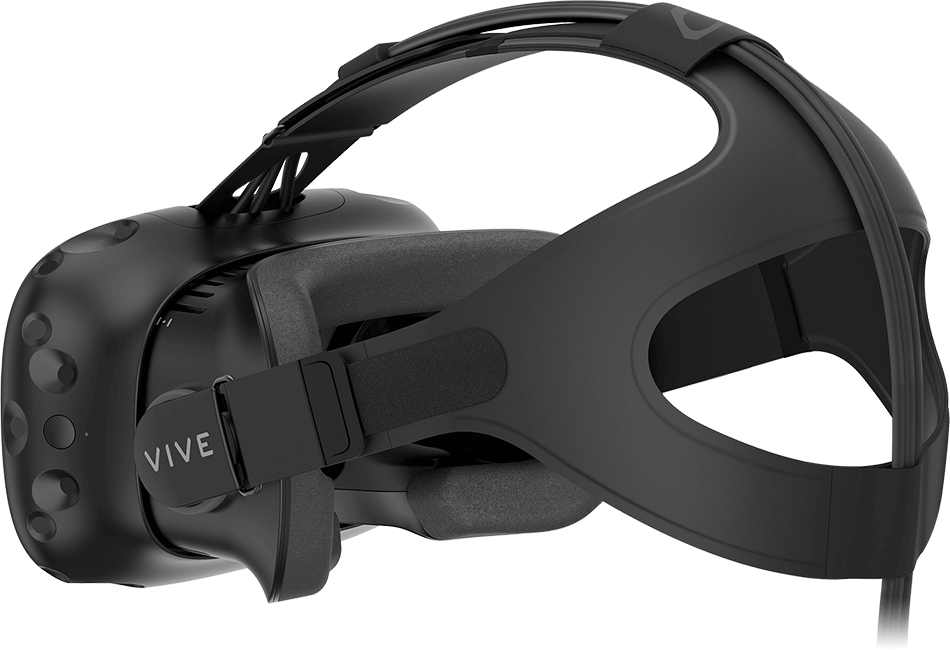
\includegraphics[width=0.5\linewidth]{vive-hardware-hmd-1}
	\caption[HMD der HTC Vive]{\acs{HMD} der HTC Vive \cite{ViveHMD}}
	\label{fig:vive-hardware-hmd-1}
\end{figure}

\subsection{Controller}
Die HTC Vive beinhaltet die in \autoref{fig:vive-hardware-controllers-1} dargestellten Controller, welche für die Interaktion in \ac{VR} verwendet werden können. Durch die Controller ist der Benutzer nicht von Maus und Tastatur abhängig, um mit der \ac{VR}-Umgebung interagieren zu können. Die Controller unterstützen haptisches Feedback mit einer hohen Auflösung, wodurch der haptische Sinn für die Immersion mit einbezogen wird. Die Controller können den Benutzer bei der Bewegung durch Teleportation in \ac{VR} unterstützen. Auf der Oberseite der Controller befindet sich ein Multifunktions-Trackpad, ein Systemknopf, eine Menütaste sowie Greifknöpfe an der Seite. Auf der Unterseite des Controllers befindet sich ein zweistufiger Abzug. \cite{ViveProduct}

\begin{figure}[!htbp]
	\centering
	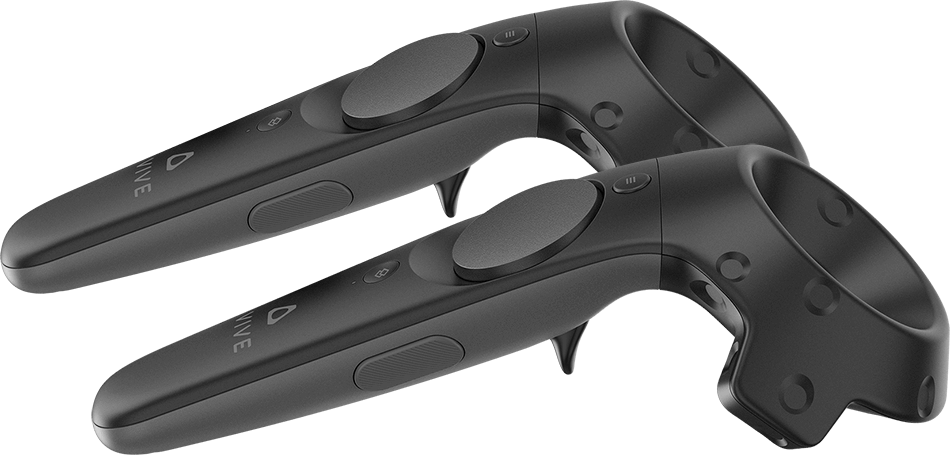
\includegraphics[width=0.5\linewidth]{vive-hardware-controllers-1}
	\caption[Controller der HTC Vive]{Controller der HTC Vive \cite{ViveControllers}}
	\label{fig:vive-hardware-controllers-1}
\end{figure}

\subsection{Tracking System}
Für das Umsehen in einer \ac{VR}-Umgebung wird ein Tracking System benötigt. Ein Tracking System erfasst die Position und die Bewegungen des Benutzers. Nach \citeauthor{Sauter.2015} unterschied sich die HTC Vive nach der Vorstellung auf der Mobile World Congress insbesondere durch das verwendete Tracking. Die Präsenz in \ac{VR} war weitaus besser als das anderer Hersteller. Während der Benutzer bei anderen Herstellern in der \ac{VR}-Umgebung stand und zuschaute, konnte der Benutzer mithilfe des Trackings der HTC Vive erstmals frei bewegen und mit der Umgebung interagieren. \cite{Sauter.2015} 

Das verwendetet Tracking System ist das von der Firma Valve entwickelte SteamVR-Tracking. Valve beschreibt SteamVR-Tracking als eine Hardware- und Softwarelösung, durch die Geräte in Echtzeit ihre Position im Raum ermitteln \cite{Valve.2020}. Während zum Beispiel bei Oculus VR kleine Infrarot-LEDs auf dem \ac{HMD} sitzen, welche von einer externen Kamera erfasst werden, verwendet SteamVR-Tracking keine Kameras\todo{meinst du hier inside out tracking von der oculus rift s oder sind das kameras die im raum stehen? wenn ja am besten den Begriff inside-out tracking benutzen, das is der fachbegriff für tracking mit kameras auf der brille selbst} \cite{Sauter.2015}. Stattdessen werden zwei Basisstationen verwendet (siehe \autoref{fig:vive-hardware-base-stations}), welche mithilfe von zwei Laserstrahlen der Klasse 1 \glqq das Zimmer mit mehreren Synchronimpulsen und Laserstrahlen im Radius von bis zu 5 Metern\grqq \cite{Valve.2020} scannen. Je ein Laser wird horizontal und vertikal rotiert. Daher wird das System auch als Lighthouse (Leuchtturm) System bezeichnet. In den zu erfassenden Objekten (zum Beispiel \ac{HMD}, Controller, etc.) sind Fotowiderstände als Sensoren integriert. Die millimetergenaue Position der Objekte wird mithilfe der integrierten Sensoren durch das Objekt selbst bestimmt. \cite{Yates.20160512}

\begin{figure}[!htbp]
	\centering
	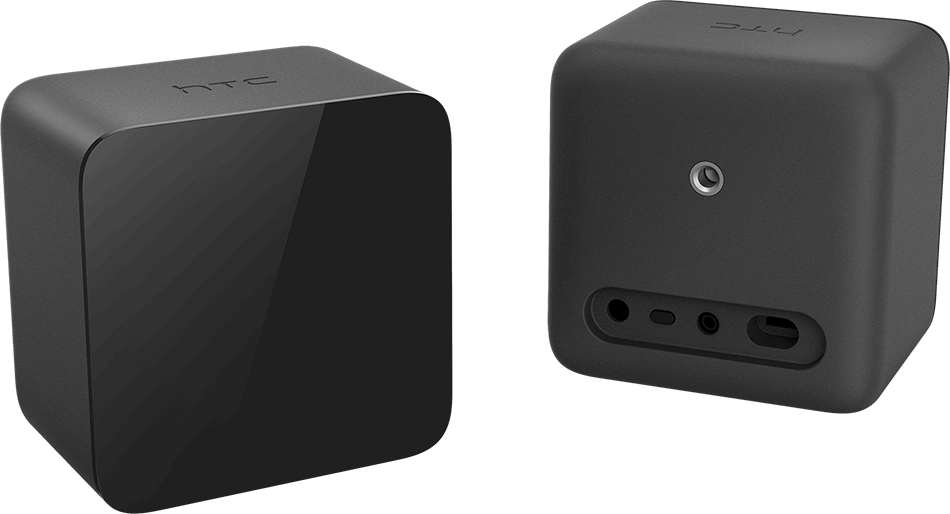
\includegraphics[width=0.5\linewidth]{vive-hardware-base-stations}
	\caption[Lighthouse Basisstationen]{Lighthouse Basisstationen \cite{ViveBaseStation}}
	\label{fig:vive-hardware-base-stations}
\end{figure}

In \autoref{fig:graphic-tracking-steamvr} ist die Funktionsweise von SteamVR-Tracking grafisch dargestellt. Die zwei Basisstationen werden gegenüberliegend an der Wand montiert. Dies ermöglicht eine 360°-Abdeckung des Raumes. Das blaue Rechteck auf dem Boden definiert den Spielbereich, in dem sich der Benutzer frei bewegen kann. Dieser Bereich wird vom Benutzer kalibriert. Die Größe ist auf maximal 15 m$^2$ begrenzt \cite{ViveProduct}. Um ein unabsichtliches Verlassen des Spielbereichs des Benutzers zu verhindern, wird der Benutzer durch das Einblenden einer Chaperone-Spielbereichsbegrenzung in Form eines Energiefeldes bei der Grenze gewarnt \cite{ViveProduct}. 

\begin{figure}[!htbp]
	\centering
	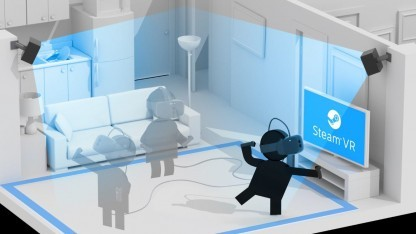
\includegraphics[width=1\linewidth]{graphic-tracking-steamvr}
	\caption[Steam VR scannt mit Lighthouse]{Steam VR scannt mit Lighthouse \cite{Sauter.2015}}
	\label{fig:graphic-tracking-steamvr}
\end{figure}

\subsection{SteamVR}
SteamVR ist eine von Valve und HTC entwickelte API, welche zusammen mit dem HTC Vive System veröffentlicht wurde. 
\todo[inline]{Muss noch geschrieben werden.}
{\color{red} SteamVR wurde von Valve und HTC als Unterstützung für Entwickler – zusammen mit dem HTC Vive System – veröffentlicht. Es bietet eine Reihe von API-Aufrufen und vorgefertigten Spiele Objekten, welche die Entwicklung von VR-Anwendungen zugänglicher gestaltet. Die Nutzung von SteamVR ist frei unter ihrer Steamworks VR API Code Lizenz}

\section{Eye-Tracking}
Eye-Tracking ist eine Technologie, welche zur Erfassung von Augenbewegungen eingesetzt wird. \citeauthor{BartlPokorny.2013} definieren Eye-Tracking wie folgt: 

\begin{quote}
	\glqq Unter Eye-Tracking versteht man die computergestützte Aufzeichnung von Augenbewegungen, welche Einsichten in perzeptuelle Verarbeitungsprozesse (vor allem Aufmerksamkeitsprozesse) und Rückschlüsse auf die Bewältigung kognitiver Aufgaben ermöglicht.\grqq \cite{BartlPokorny.2013} 
\end{quote}

Die wichtigsten Parameter, die durch das Eyetracking erfasst werden, sind Fixiationen, Sakkaden und Regression \cite{BartlPokorny.2013}. \glqq Fixationen sind Phasen des relativen Stillstandes der Augen.\grqq \cite{Blake.2013} Als Sakkaden werden schnelle Augenbewegungen bei der Erfassung eines neuen Fixpunktes bezeichnet. Regressionen bezeichnen Richtungsänderungen und Rücksprünge zu vorherigen Fixpunkte. Die verfügbaren Systeme lassen sich in drei Gruppen unterteilen: Fixierung am Kopf (tower-mounted) \todo{head-mounted klingt für mich auch nach fixierung am kopf, hier vlt ein wenig klarer formulieren}, berührungslose Messung (remote) und sowie mobiles Eye-Tracking (head-mounted). \cite{BartlPokorny.2013}
\todo[inline]{Noch darauf eingehen, wie Eye-Tracking technisch funktioniert???}

\subsection{Eyetracker}
Im Rahmen dieser Arbeit wird die Eye-Tracking Plattform von Pupil Labs verwendet. Die Firma entwickelt seit 2014 die Plattform Pupil Core, welche Eyetracker und eine Open-Source-Software-Suite beinhaltet. In \autoref{fig:pupil_labs_headset} ist das mobile Eye-Tracking Headset Pupil Core zu sehen. An dem Headset ist eine Umgebungskamera (Nummer 1) angebracht, welche das Blickfeld des Benutzers aufzeichnet. Zudem wird eine Infrarot-Spektrum-Augenkamera (Nummer 3) zur Erkennung \todo{sind die nicht immer dunkel? :D; Naja steht so in der Quelle :D}dunkler Pupillen eingesetzt \cite{Kassner_2014}. Die Kameras sind individuell einstellbar, um eine optimale Erfassung des Auges zu gewährleisten. Jedes Auge wird mit einer Frequenz von 200 Hz und einer Auflösung von \mbox{192 x 192} Pixel erfasst \cite{PupilLabsSpec}. Ein USB-C Kabel (Nummer 4) dient zur Stromversorgung und für den Austausch der Videodaten der Kameras mit einem Computer. Die Open-Source-Software-Suite lässt sich nach \citeauthor{Kassner_2014} in zwei Hauptteile aufteilen: Pupil Capture und Pupil Player. Pupil Capture erfasst und verarbeitet die Videodaten der Kameras in Echtzeit. Zudem lassen sich die Daten aufzeichnen, welche mit Pupil Player wiedergegeben sowie visualisiert werden. Der verwendete Algorithmus zur Erkennung der Pupille lokalisiert die dunkle Pupille im Bild der Augenkamera. In den meisten Umgebungen ist der Algorithmus robust gegenüber Reflexionen im Pupillenbereich. Zudem benötigt der Algorithmus nicht die Hornhautreflexion und funktioniert bei Anwendern, die sowohl Kontaktlinsen als auch Brillen tragen. \cite{Kassner_2014} Bei Bedarf kann über eine Netzwerkschnittstelle mit Pupil Capture interagiert werden. Es ist möglich, Daten zu empfangen und an Pupil Capture zu senden. \cite{PupilLabsNet} Die Genauigkeit des Eyetrackers wird mit 0,6° angegeben \cite{PupilLabsSpec}.

\begin{figure}[!htbp]
	\centering
	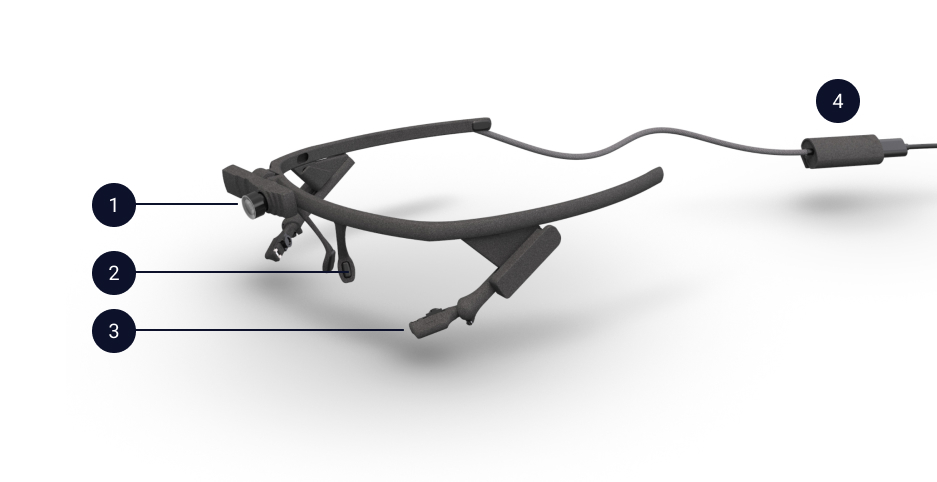
\includegraphics[width=0.75\linewidth]{pupil_labs_headset}
	\caption[Pupil Core Headset]{Pupil Core Headset \cite{PupilLabsHW}}
	\label{fig:pupil_labs_headset}
\end{figure}

\subsection{Kalibrierung}
Die Kalibrierung ist ein Verfahren, um die Genauigkeit von Eye-Tracking zu gewährleisten \cite{Clay_Koenig_Koenig_2019}. Die Durchführung findet durch Betrachtung einer vordefinierten Anzahl visueller Stimuli statt, welcher der Benutzer während der Kalibrierung anvisieren muss. Während des Anvisierens der Zielpunkte werden die Pupillenposition im Augenbild, die physische Orientierung des Auges und die Lage des Ziels auf der Kalibrierungsebene abgetastet. \cite{Lander.2018} Aus diesen Informationen wird der Blick an die Stelle angepasst, an die der Benutzer schaut \cite{Clay_Koenig_Koenig_2019}. Das Kalibrieren ist ein individueller Prozess, weshalb das Eye-Tracking vor der Anwendung für jeden Benutzer neu kalibriert werden muss. Der Grund sind unter anderem die humanspezifischen Parameter (zum Beispiel Hornhautverkrümmung), und geometrischen Informationen (zum Beispiel relative Lage und Orientierung zwischen den Kameras). \cite{Lander.2018}

Während der Kalibrierung verwendet der Eye-Tracker diese Zielpunkte als Referenzpunkte, um seine Berechnung des Blicks an die Stelle anzupassen, auf die die Testperson schaut. 

Pupil Capture bietet hauptsächlich zwei verschiedene Methoden zur Kalibrierung an. Die erste Methode eignet sich für Eye-Tracking im Nahbereich in einem engen Sichtfeld. In \autoref{fig:CalibrationMarker-2D} ist die erste Möglichkeit abgebildet. Eine Zielscheibe befindet sich in der Mitte, die anderen vier je in der Ecke des Bildschirmes. Wenn ein Stimulus angezeigt wird, werden die anderen Stimuli ausgeblendet. Diese Methode wird standardmäßig verwendet. Die zweite Möglichkeit eignet sich für mittlere Entfernungen und einem breiten Sichtfeld. Hier wird der Stimulus auf zum Beispiel einem Blattpapier vor den Benutzer gehalten. Pupil Capture erkennt den Stimulus über die Umgebungskamera. Hierfür ist es notwendig, dass der Stimulus dem Kalibrierungsmarker, in Form der Zielscheibe, entspricht. Beide Möglichkeiten können zudem nur mit einem Stimulus durchgeführt werden. \cite{PupilLabsCalib}

Nach \citeauthor{Lander.2018} wird die Genauigkeit von Eye-Tracking aufgrund von Kalibrierdrift immer schlechter. Daraus folgt, dass eine regelmäßige Neukalibrierung für eine genaue Blickschätzung benötigt wird. \cite{Lander.2018} Gründe sind Veränderungen der Augenphysiologie (zum Beispiel Nässe des Auges), der Umgebung (zum Beispiel Lichtverhältnisse), die Position des Gerätes oder der Kamera in Bezug auf das Auge sowie des Standortes und der Orientierung des Benutzers \cite{Cerrolaza.2012}. \citeauthor{Clay_Koenig_Koenig_2019} empfehlen bei Experimenten das Kalibrieren alle fünf bis zehn Minuten zu wiederholen \cite{Clay_Koenig_Koenig_2019}. 

\begin{figure}[!htbp]
	\centering
	\fbox{
\includegraphics[width=1.0\linewidth]{CalibrationMarker-2D}}
	\caption[Anordnung der Zielpunkte während der Kalibrierung von Pupil Core]{Anordnung der Zielpunkte während der Kalibrierung von Pupil Core (Zielpunkte von \cite{PupilLabsCalibMarker})}
	\label{fig:CalibrationMarker-2D}
\end{figure}

\subsection{Eye-Tracking in VR}
Da in dieser Arbeit das Eyetracking innerhalb einer \ac{VR}-Umgebung untersucht wird, wird ein speziell für die HTC Vive entwickelter Eyetracker von Pupil Labs verwendet. Dies ist ein Add-on von Pupil Labs, welches in das \ac{VR}-Headset HTC Vive eingebaut wird. In \autoref{fig:pupil_labs_addon} ist das Add-on von Pupil Labs und das \ac{VR}-Headset HTC Vive dargestellt. Das Add-on wird in die Innenseite um die Linsen des Headsets angebracht. Das Add-on ist im Vergleich zu dem Eyetracker-Headset fast identisch. Die Genauigkeit ist jedoch schlechter als beim Eyetracker-Headset. Sie beträgt beim Add-on ca. 1° \cite{PupilLabsAddOnSpecs}. Zudem entfällt die Umgebungskamera beim Eyetracker komplett. 

\begin{figure}[!htbp]
	\centering
	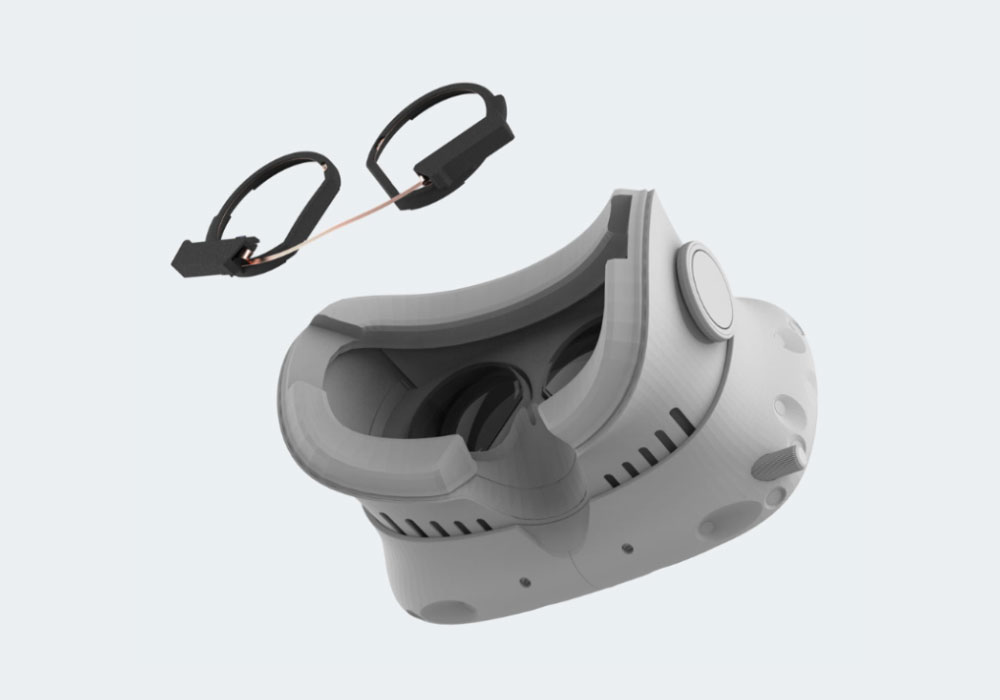
\includegraphics[width=0.75\linewidth]{vive-addon}
	\caption[Pupil Core Add-on für HTC Vive]{Pupil Core Add-on für HTC Vive \cite{PupilLabsAddOn}}
	\label{fig:pupil_labs_addon}
\end{figure}

Die Funktionsweise des Eye-Trackings in der realen Welt ist nicht komplett auf die virtuelle Welt übertragbar. Nach \citeauthor{Clay_Koenig_Koenig_2019} ist es daher wichtig die Fixierungspunkte bei der Kalibrierung im Bildschirmraum und nicht im \ac{VR}-Weltraum darzustellen\todo{ist das nicht logisch? also ich würde da nicht unbedingt die Leute zitieren, das sollte eigentlich klar sein, dass man in VR keine echten punkte zur Kalibrierung nehmen kann. Hört sich komisch an wenn man sich dafür auf Leute beziehen muss}. Die Fixierungspunkte bewegen sich zusammen mit dem Kopf des Benutzers, weshalb der Benutzer die Fixierungspunkte nicht durch Kopfbewegungen ins Zentrum des Sichtfeldes bekommt. Alle Ziele bleiben daher an ihrer vorgesehenen Position und das gesamte Sichtfeld wird für das Eye-Tracking kalibriert. Da die Auflösung von der Mitte bis zum Rand des Sichtfeldes schlechter wird \cite{Kreylos.2017}, sollte bei der Kalibrierung der Fokus auf die Mitte des Sichtfeldes liegen. Der Benutzer muss seine Augen nicht zu weiten Exzentrizitäten bewegen, sondern kann sein Kopf dem Objekt zuwenden, welches dieser beobachten möchte. Deshalb ist es sinnvoll eine höhere Genauigkeit in Bereichen des stärksten Sehens des Sichtfeldes zu gewährleisten. \cite{Clay_Koenig_Koenig_2019} \\ 
Im Gegensatz zu einem Eyetracker mit Umgebungskamera müssen die erfassten 2D-Blickdaten in 3D-Blickdaten für \ac{VR}-Umgebung konvertiert werden. Bei einem Eyetracker bewegt sich die Umgebungskamera mit der Bewegung des Kopfes mit. Das bedeutet, dass die Umgebungskamera immer in der selben Position in Relation zu den Augen steht. Die 2D-Blickdaten können daher in das aktuelle Umgebungsbild hinzugefügt werden. In \ac{VR} muss ein 3D-Blickvektor berechnet werden. Dieser setzt sich aus den 2D-Blickdaten und der Position des Kopfes zusammen. \cite{Clay_Koenig_Koenig_2019}

\section{Unity}
Standardmäßig entspricht 1 Einheit 1 Meter (siehe \cite{BrentAllard.2017} \& \cite{AVividLight.2010}) --> Aussage ist plausibel, da standardmäßig in den Projekteinstellungen bei Physics die Gravitation auf -9,81 gesetzt ist.

Objekt Lebenszyklus; Start, Awake usw.

Screenspace - overlay; screenspace - camera, worldspace

GameObject, Collider, Component, Canvas, usw.

\subsection{Plugins}
Hier eine Einführung in Plugins in Unity geben. Danach Überleitung zu den verwendeten Plugins steamVR und hmd\_eyes.

\subsubsection{steamVR}

\subsubsection{hmd\_eyes}


\section{Fitts' Gesetz}
Fitts' Gesetz (im englischen Fitts's Law) ist eine vom US-Amerikanischen Psychologe Paul Morris Fitts im Jahre 1954 veröffentlichte Metrik, welche die Schwierigkeit des Bewegens eines Objektes an eine bestimmte Stelle numerisch beschreibt. \citeauthor{Fitts.1992} hat in seiner Veröffentlichung ein Experiment beschrieben, in dem Probanden einen Gegenstand entlang einer Linie in einen Zielbereich bewegen sollen. Numerische Parameter zur Bestimmung des \glqq Index of Difficulty\grqq{} (Index der Schwierigkeit) sind zum einen die Distanz D zum Zielbereich und die Breite des Zielbereiches W \cite{Fitts.1992}.
\begin{equation}
ID = log_2 \left ( \frac{2D}{W} \right )
\end{equation}
Eine Erhöhung der Distanz hat eine Erhöhung der Schwierigkeit zur Folge, wohingegen eine Erhöhung der Breite das Senken des Schwierigkeitsindex ID zur Folge hat. Ein niedriger Wert für ID bedeutet, dass das Objekt leicht zu treffen ist, ein hoher Wert bedeutet, dass das Objekt schwer zu treffen ist \cite{Fitts.1992}. 
Basierend auf dieser Berechnung ist es möglich, die Bewegungsdauer MT (Movement Time) zu berechnen. Die Berechnung von MT ist nach \citeauthor{Graham.1996} mit folgender Formel möglich \cite{Graham.1996} \todo{vlt gibts die Quelle iwo anders besser... so is nur mittelmäßig nice}:
\begin{equation}
MT = a + b * ID = a + b * log_2 \left ( \frac{2D}{W} \right )
\end{equation}
Die Konstanten a und b sind Zeitkonstanten, die von dem verwendeten Eingabegerät abhängig sind. Dabei beschreibt a die Zeit, bis eine Bewegung beginnt und b die Beschleunigungskonstante. Daher wird mit einer erhöhten Distanz die Zeit, bis das Objekt ausgewählt wird, ebenfalls höher \cite{Graham.1996}. {\color{red} Daher erhöht sich die Zeit, bis das Objekt ausgewählt wird, sobald sich die Distanz erhöht \todo{Alternative zum Satz davor}}

Mittlerweile wird sich vor allem in der Erstellung von Benutzeroberflächen auf Computerbildschirmen (User Interfaces, kurz UIs) an den Erkenntnissen von Fitts  orientiert, um Schaltflächen für Nutzereingaben möglichst so zu gestalten, dass sie schnell und einfach getroffen werden können \cite{Kexugit.2006}. Durch die begrenzte Fläche auf einem Computerbildschirm bietet sich hier ebenfalls die Möglichkeit, an den Rändern des Bildschirms wichtige Bedienelemente zu platzieren, um eine schnellere Bedienung des Programms vornehmen zu können. Im Betriebssystem Windows 10 ist zum Beispiel der Startknopf in der unteren linken Ecke, der sogenannten \glqq Magic Corner \grqq{} platziert \cite{Kexugit.2006}. Dadurch hat dieser Knopf eine \glqq unendliche\grqq{} Höhe und Tiefe, da der Nutzer die Maus unendlich weit nach unten links bewegen kann und immer den Startknopf treffen wird \cite{Kexugit.2006}. Dadurch wird die Zeit, bis ein Nutzer den Knopf getroffen hat und aktivieren kann deutlich reduziert \cite{Soukoreff.2004}.

Bei Experimenten mit Fitts' Gesetz werden sowohl die Breite W und die Distanz D variiert, jedoch sollten die beiden Parameter nicht gleichzeitig variiert werden, um eine genauere Aussagekraft zu erlangen. 

Da Fitts das Ursprungsexperiment ausschließlich in einer Dimension durchgeführt hat, war es ausreichend, ausschließlich die Breite des Zielbereichs als Breite W zu nutzen. Da aber ein Computerbildschirm zweidimensional ist, muss der Parameter angepasst werden, um die zweite Dimension ebenfalls in W darzustellen. Ansätze hierfür sind beispielsweise die Fläche des Objekts als W zu nutzen, oder die Breite mit der Höhe zu addieren. Da diese Ansätze aber nicht die Bewegungsrichtung beachten, wird in den meisten Fällen die Länge des Objekts in Bewegungsrichtung verwendet. Deshalb werden in den meisten Untersuchungen zu dem Thema Kreise verwendet, da hier W unabhängig von der Bewegungsrichtung konstant ist \cite{Soukoreff.2004}. 

\subsection{Fitts' Gesetz und Eye-Tracking}
Bei Eye-Tracking Steuerung wird weiterhin diskutiert, ob Fitts' Gesetz weiterhin einsetzbar ist. Eine weite Bewegung mit dem Auge zeichnet sich, im Gegensatz zu einer weiten Bewegung mit der Maus, nicht über die zurückgelegte Distanz, sondern über den Winkel zwischen zwei Objekten aus. Unter Berücksichtigung dieses Aspekts ist es aber möglich, Fitts' Gesetz anzuwenden. Allerdings können hier Ungenauigkeiten auftreten, die z.b. bei der Steuerung mit einer Maus nicht auftreten können. Dies kann zum Beispiel durch Bewegungen des gesamten Kopfes und nicht nur der Augen geschehen. Allgemein hat \citeauthor{Miniotas.2000} belegt, dass eine Übertragung von Fitts' Gesetz zu Eye-Tracking möglich ist. \cite{Miniotas.2000}

\subsection{Fitts' Gesetz und Virual Reality}
Bei der Erstellung einer Nutzeroberfläche in der virtuellen Realität ist Fitts' Gesetz grundsätzlich weiterhin anwendbar. Dies haben \citeauthor{Hansen.2018} in einem Vergleich von Maussteuerung, Kopfsteuerung und Blicksteuerung gezeigt.\cite{Hansen.2018} Allerdings ist hier die Distanz zwischen zwei Punkten durch die komplette Immersion des Nutzers in der virtuellen Welt besser durch die Verwendung von Winkeln, als der Verwendung von Pixeln als Maßeinheit anzugeben \cite{Hansen.2018}. Für ein vergleichbares Ergebnis ist es hier jedoch wichtig, dass die Kopfposition möglichst fixiert ist. Durch eine festgesetzte Position des Nutzers ist der Winkel zwischen zwei Objekten immer der Selbe und somit die Bewegung eines Zeigers in Form eines Laserpointers oder des Blicks immer mit der gleichen Bewegungslänge verbunden. Dies gilt auch für die Breite eines Objektes. Allerdings können sich diese Werte durch unbeabsichtigt, beziehungsweise intuitiv stattfindende Kopfbewegungen ebenfalls wieder verändern. Dies ist nur bedingt kontrollierbar und kann deswegen zu Verzerrungen in den Ergebnissen führen. 

\subsection{Fitts' Gesetz mit Eye-Tracking in Virtual Reality}
Wenn man die Erkenntnisse der beiden vorherigen Abschnitten zusammenführt, ergibt sich eine Situation, in der Fitts' Gesetz in VR mit Eye-Tracking durchaus überprüft werden kann. Allerdings müssen einige Parameter, wie beispielsweise die Distanz zu den Objekten fest definiert sein. \citeauthor{Hansen.2018} haben in ihrer Untersuchung bereits VR und Eye-Tracking verbunden und sind zu dem Schluss gekommen, dass es als Steuermöglichkeit durchaus Potential hat, allerdings immer noch der herkömmlichen Computermaus unterlegen ist. \cite{Hansen.2018}

\section{Systemvoraussetzung}
\todo[inline]{Systemvoraussetzungen mit rein nehmen???? -> wie besprochen, auch die min specs von der Vive Seite mit rein nehmen \& Pupil Labs}
Verwendete Hardware: i5 8600k, gtx 1060 6gb, 16gb ddr4

\begin{figure}[!htbp]
	\centering
	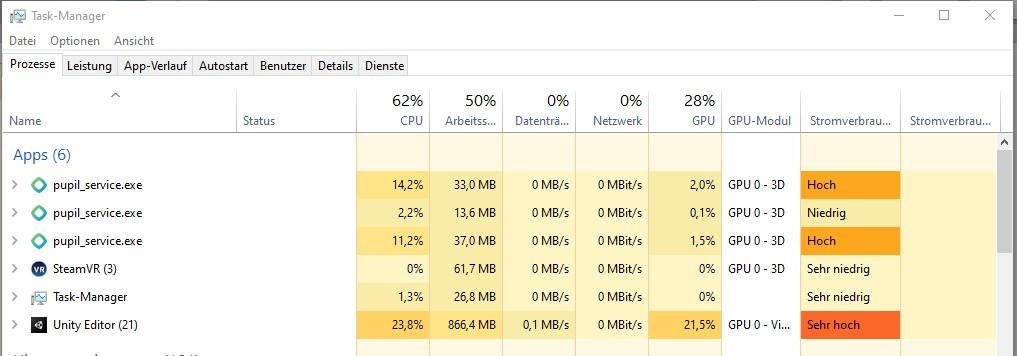
\includegraphics[width=1\linewidth]{Systemauslastung}
	\caption[Systemauslastung]{Systemauslastung}
	\label{fig:Systemauslastung}
\end{figure}